\chapter{Experimental Setup}

\section{Coil Design}

We have designed a Helmholtz Coil on SolidWorks with a radius of $40mm$, width of $9mm$ and $30$ turns. 

\begin{figure}[h]
    \centering
    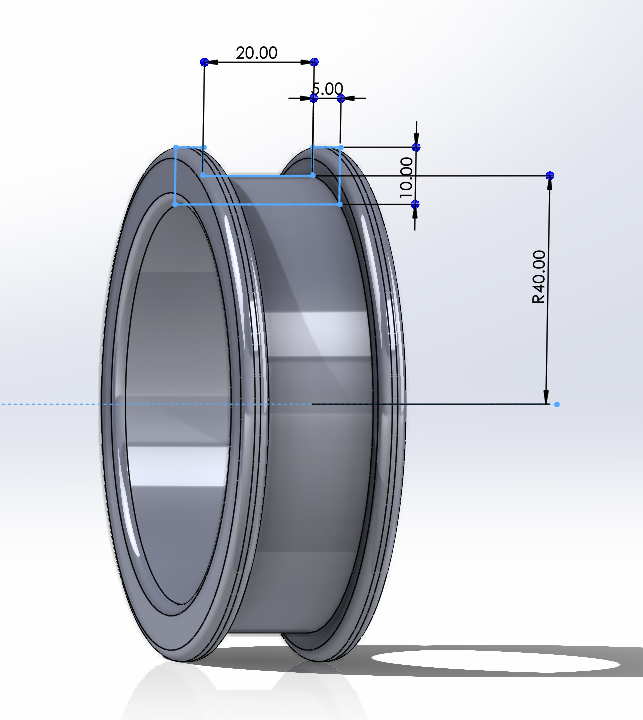
\includegraphics[width=0.4\textwidth]{assets/coil-design-single.png}
    \caption{Coil Design}
    \label{fig:helmholtz-coil}
\end{figure}

And we have 3D printed the coil design with PLA filament.

\begin{figure}[h]
    \centering
    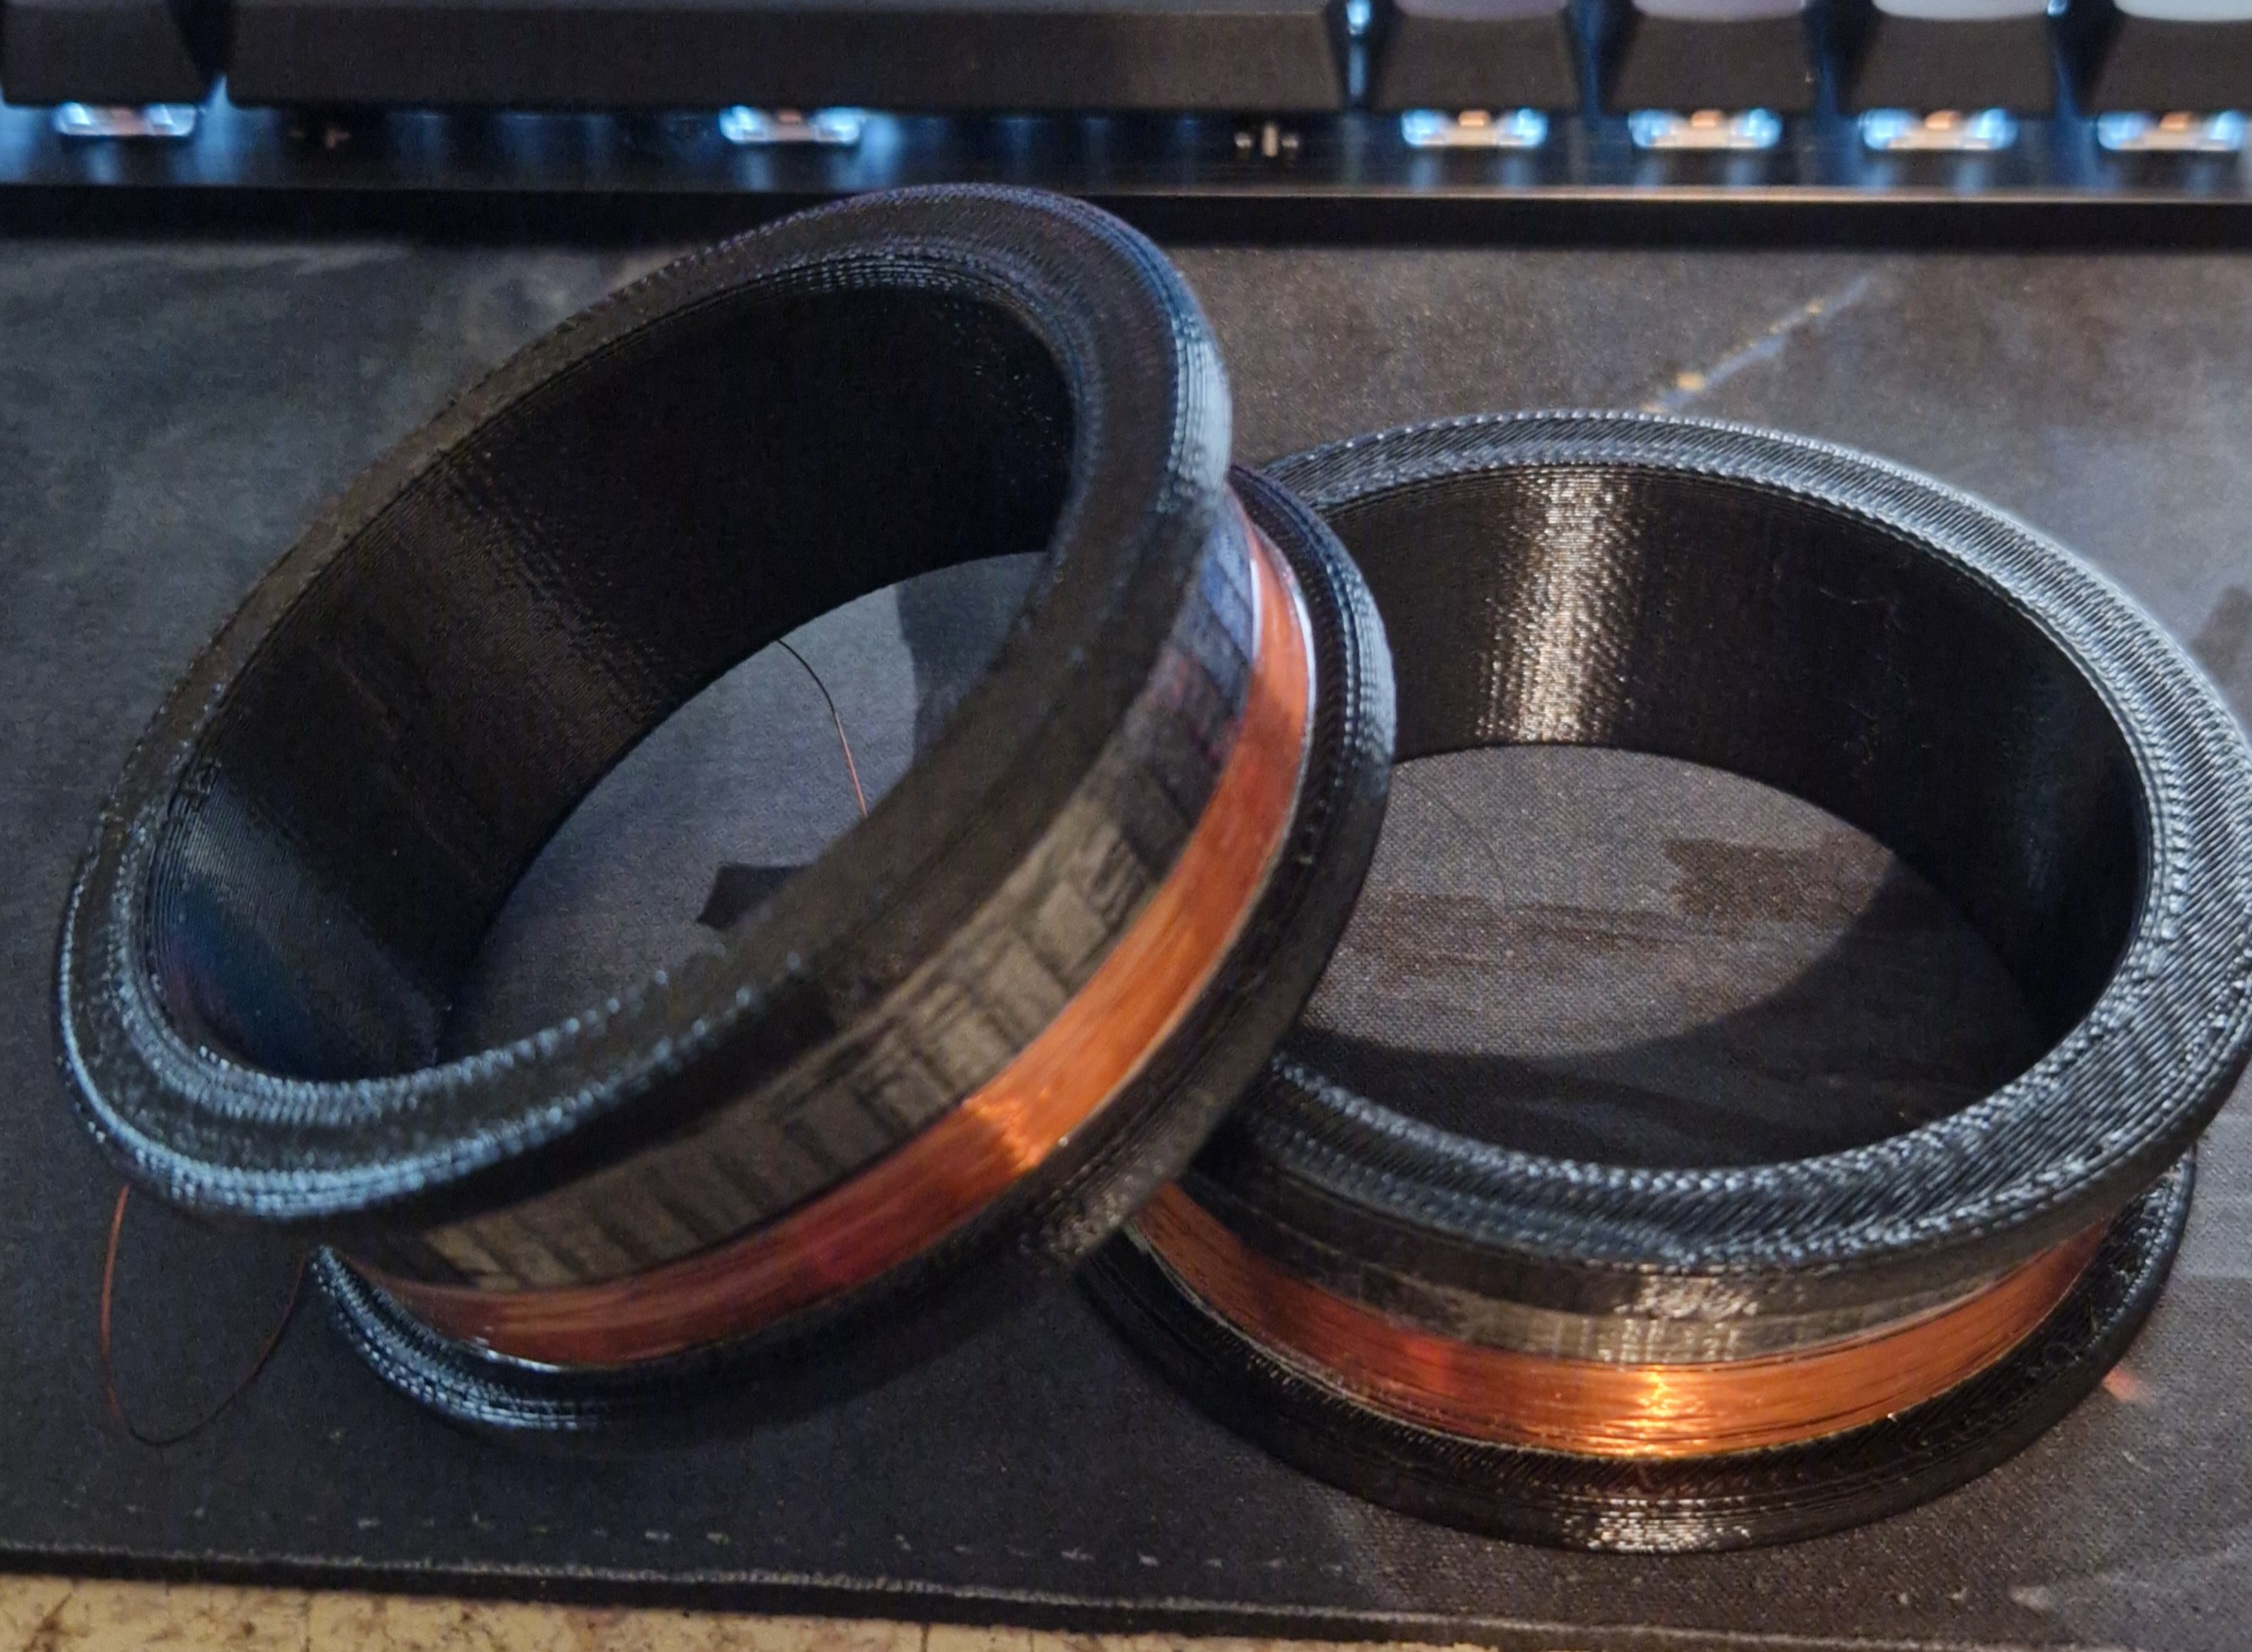
\includegraphics[width=0.4\textwidth]{assets/3d-printed-coil.jpg}
    \caption{3D Printed Coils}
    \label{fig:helmholtz-coil-3d-printed}
\end{figure}

\newpage{}
\thispagestyle{plain}

Also created a board to connect the coils to the circuit easliy. In next steps, we'll use more than one resistor and inductor, so we have designed the board to connect them easily.

\begin{figure}[h]
    \centering
    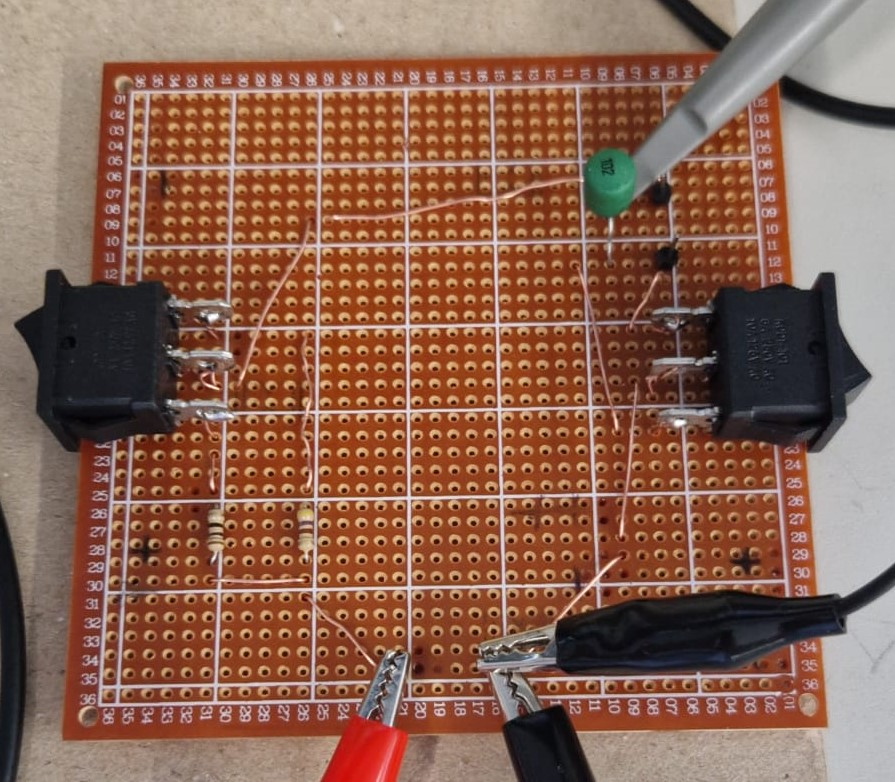
\includegraphics[width=0.3\textwidth]{assets/prototype-board.jpg}
    \caption{Prototype Board}
    \label{fig:prototype-board}
\end{figure}

\section{Measurement System}

We set up a simple RL circuit using our 3D printed coils. Used a $470\Omega (466\Omega)$ resistor and a sinusodial wave generator at $4V_{pp}(4.16V_{pp})$ $1kHz$ frequency.   

% draw the circuit diagram
\begin{figure}[h]
    \centering
    \begin{circuitikz}
        \draw (0,0) to[sinusoidal voltage source, l=$V_{in}$] (0,4)
        to[R, l=$R$] (4,4)
        to[L, l=$L$] (4,0)
        to[short] (0,0);
    \end{circuitikz}
    \caption{RL Circuit}
    \label{fig:rl-circuit}
\end{figure}

And divided input and output voltages. To find the inductance of the coil, we made circuit analysis in phasor domain and used the following formula:

\begin{align*}
    v_{out} &= L \cdot \frac{\partial i}{\partial t} \Rightarrow V_{out}(\omega) = Lj\omega I \\
    I &= \frac{V_{in}}{R + j\omega L} \\
    V_{out} &= Lj\omega \cdot \frac{V_{in}}{R + j\omega L} \\
    \frac{V_{out}}{V_{in}} &= \frac{Lj\omega}{R + j\omega L} \Rightarrow \frac{|V_{out}|}{|V_{in}|} = \frac{\omega L}{\sqrt{R^2 + \omega^2L^2}} \\
    &\boxed{\frac{|V_{out}|}{|V_{in}|} = \frac{2\pi f L}{\sqrt{R^2 + (2\pi f L)^2}}} \\
\end{align*}

\newpage{}
\thispagestyle{plain}

\subsection{System Validation}
To validate the system, we used a $1mH$ inductor and measured the output voltage. Signal generator set to $1kHz$ frequency and $4V_{pp}$ amplitude. Even thoug we set the input voltage to $4V_{pp}$, we red $4.16V_{pp}$ on the oscilloscope: 

\begin{figure}[h]
    \centering
    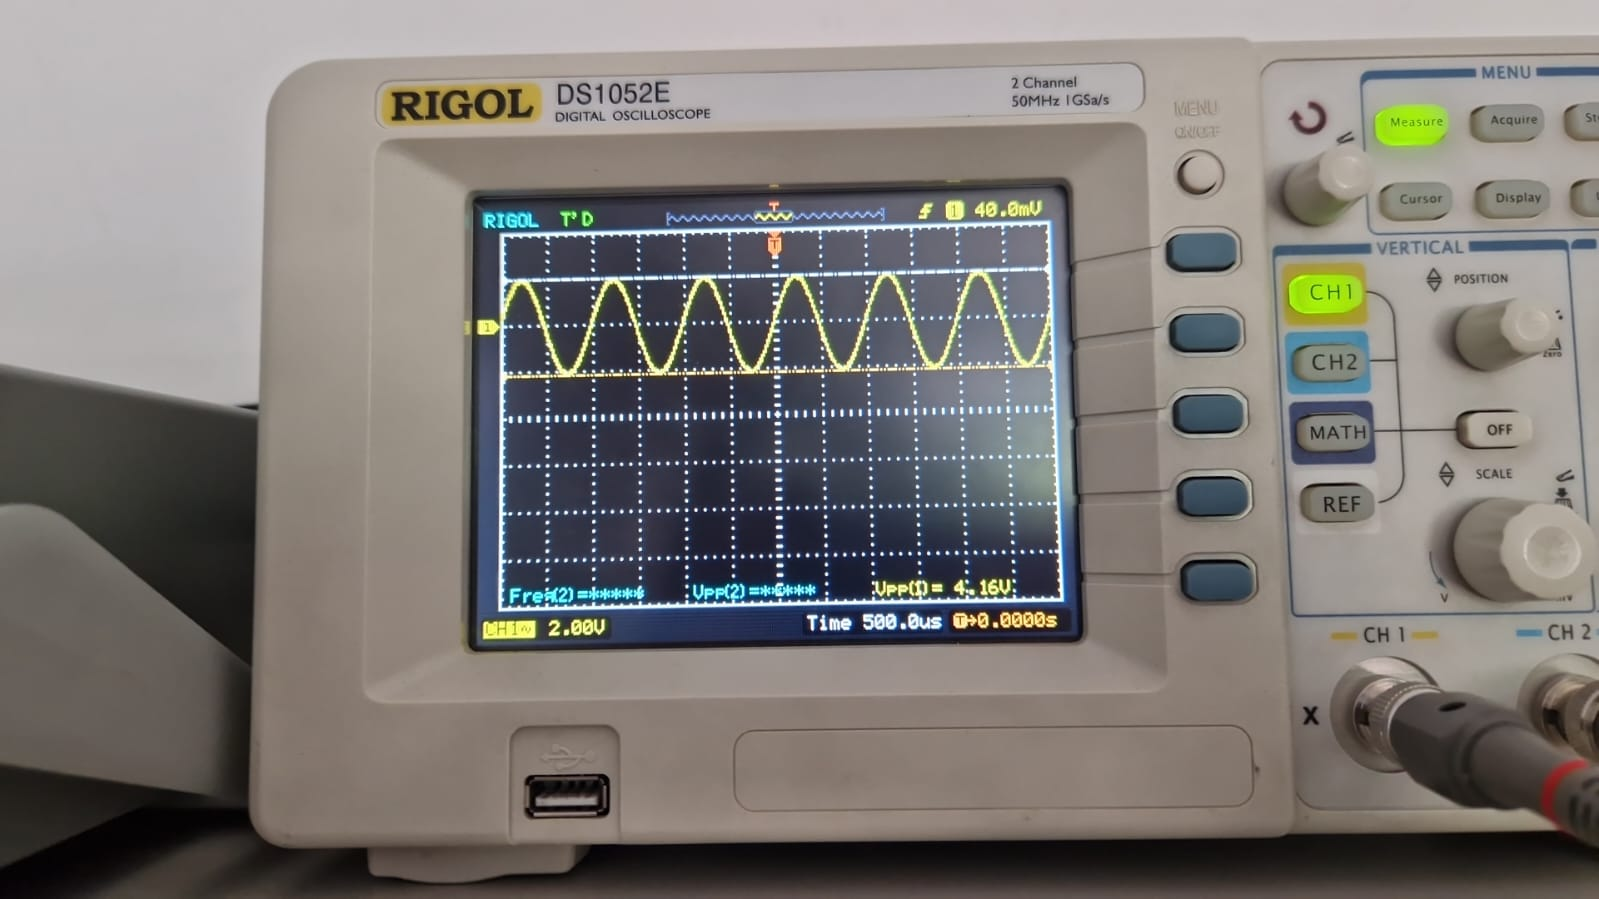
\includegraphics[width=0.9\textwidth]{assets/1k-input.jpg}
    \caption{$4V_{pp}$ Signal Generator Output}
    \label{fig:1k-signal-generator-output}
\end{figure}

And connected the $1mH$ inductor to the circuit and measured the output voltage:

\begin{figure}[h]
    \centering
    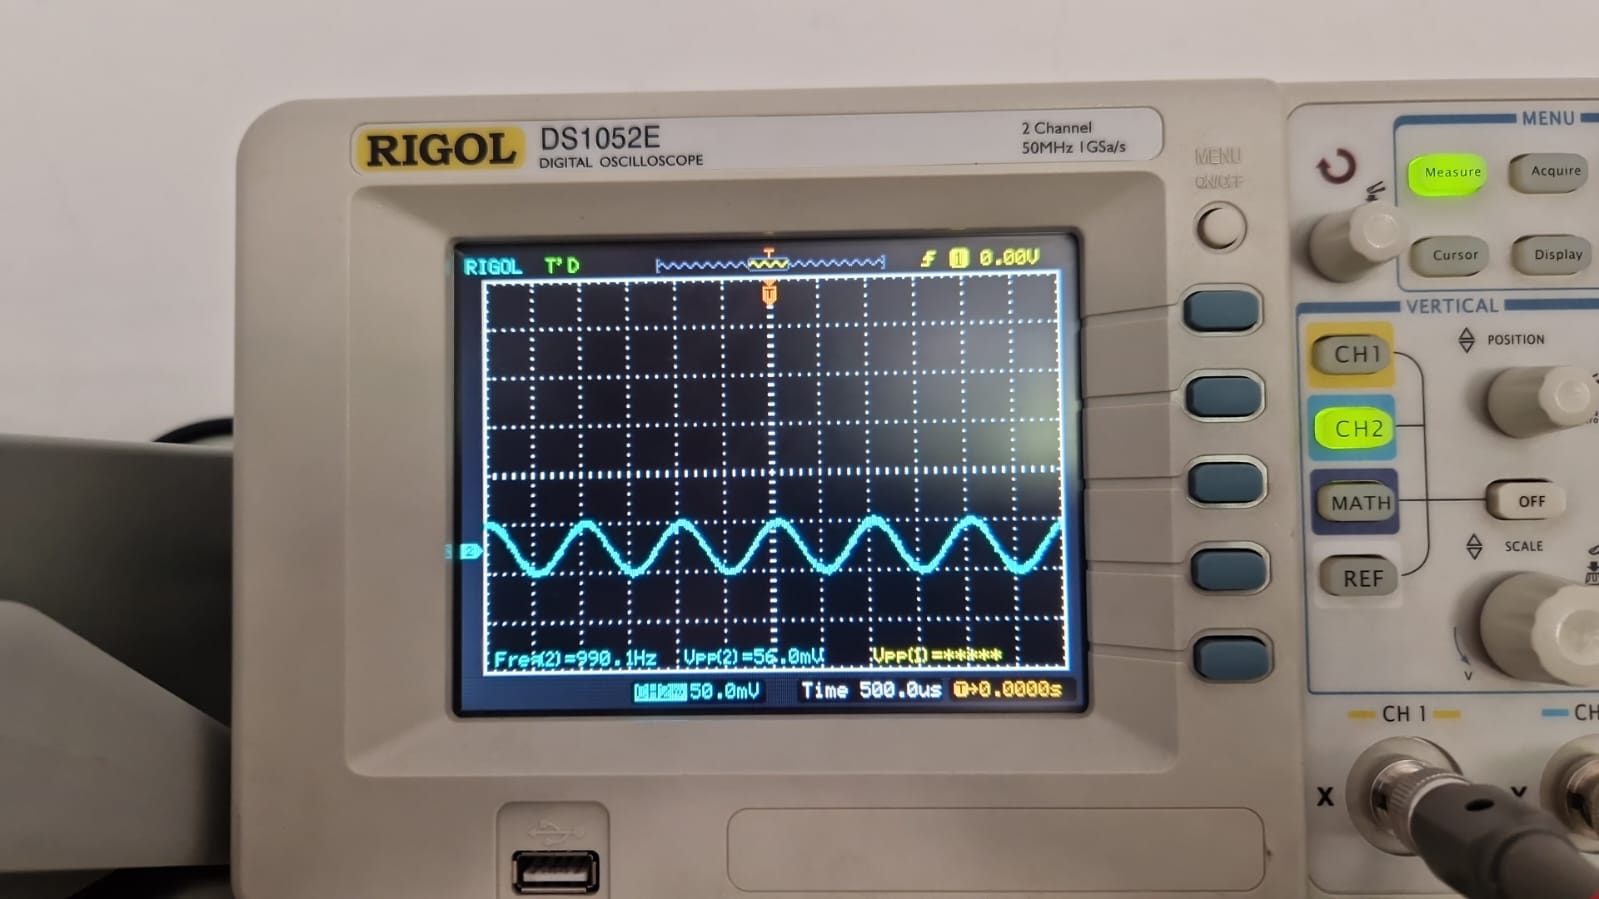
\includegraphics[width=0.9\textwidth]{assets/1k-1m-output.jpeg}
    \caption{1mH Inductor Output}
    \label{fig:1k-1m-output}
\end{figure}

\newpage{}
\thispagestyle{plain}

After putting every value to the formula, we found the inductance of the coil as follows:

\begin{align*}
    \frac{|V_{out}|}{|V_{in}|} &= \frac{2\pi f L}{\sqrt{R^2 + (2\pi f L)^2}} \\
    \Rightarrow \frac{27 \cdot 10^{-3}}{213 \cdot 10^{-2}} &= \frac{2\pi \cdot 10^3 \cdot L}{\sqrt{466^2 + (2\pi \cdot 10^3 \cdot L)^2}} \\
    L &\approx 0.00094H \approx 0.94mH
\end{align*}

It is very close to the actual value of the inductor, so we can say that our system and theoretical calculation is working properly.

\section{Calculating the Inductance of the Helmholtz Coil}

\subsection{Theoretical Calculation}

The inductance of a Helmholtz coil can be calculated using the following formula:

\[ L = \frac{\mu N^2A}{l} \]

\noindent Where:
\begin{itemize}
    \item \( \mu \) is the permeability of the air ($4\pi \cdot 10^{-7}H/m$, \cite{air_permeability_saini})
    \item \( N \) is the number of windings
    \item \( A \) is the area of the coil
    \item \( l \) is the length of the coil
\end{itemize}

According to the formula, the inductance of the Helmholtz coil is calculated as follows:

\begin{align*}
    L &= \frac{4\pi \times 10^{-7} \times 30^2 \times \pi \times 0.04^2}{0.009} \\
    &\approx 0.00063H \approx 0.63mH~\text{For one coil} \\
    &\approx 0.00126H \approx 1.26mH~\text{For two coils}
\end{align*}

\newpage{}
\thispagestyle{plain}

\subsection{Experimental Calculation}

The theoretical inductance of Helmholtz Coil is \( 1.26mH \). To find the real inductance, we changed the $1mH$ inductor from the circuit before and connected the Helmholtz coil to the circuit. Input voltage, resistor and frequency are the same as the previous experiment. Output voltage is as follows:

\begin{figure}[h]
    \centering
    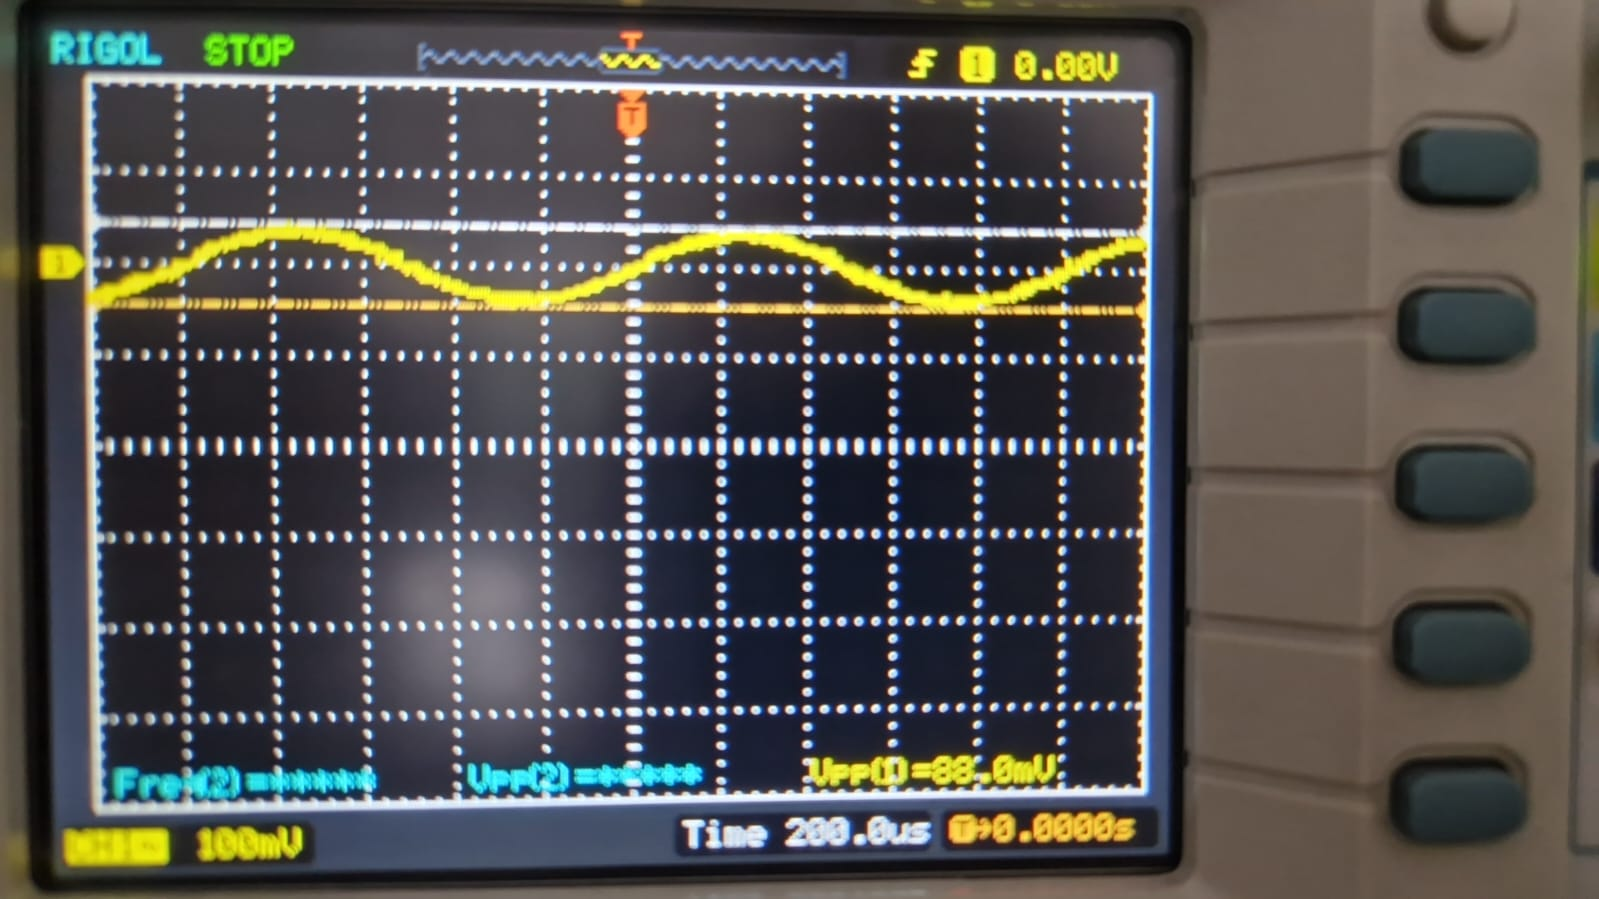
\includegraphics[width=0.9\textwidth]{assets/1k-helmholtz-output.jpg}
    \caption{Helmholtz Coil Output}
    \label{fig:1k-helmholtz-output}
\end{figure}

Output reads $88mV_{pp}$ on the oscilloscope. After putting every value to the formula, we found the inductance of the coil as follows:

\begin{align*}
    \frac{|V_{out}|}{|V_{in}|} &= \frac{2\pi f L}{\sqrt{R^2 + (2\pi f L)^2}} \\
    \Rightarrow \frac{44 \cdot 10^{-3}}{213 \cdot 10^{-2}} &= \frac{2\pi \cdot 10^3 \cdot L}{\sqrt{466^2 + (2\pi \cdot 10^3 \cdot L)^2}} \\
    L &\approx 0.00153H \approx 1.53mH
\end{align*}

Real inductance is \( 1.53mH \) which is very close to the theoretical value $1.26mH$. We can say that our system is working properly. Difference between the theoretical and experimental values can be due to the imperfections in the coil design and different magnetic properties of the materials used in the coil.

Now we are about to analyze the frequency response of the RL circuit with the Helmholtz coil with the following frequencies:

\begin{align*}
    f &= 1/T \\
    T &= 10L/R = 0.0015s \implies f = 666Hz \\
    T &= L/R = 0.00015s \implies f = 6.66kHz \\
    T &= L/10R = 0.000015s \implies f = 66.66kHz
\end{align*}

\newpage{}
\thispagestyle{plain}

\subsection{Frequency Analysis}

\subsubsection{T=10L/R $\implies$ f=666Hz}

\begin{figure}[h]
    \centering
    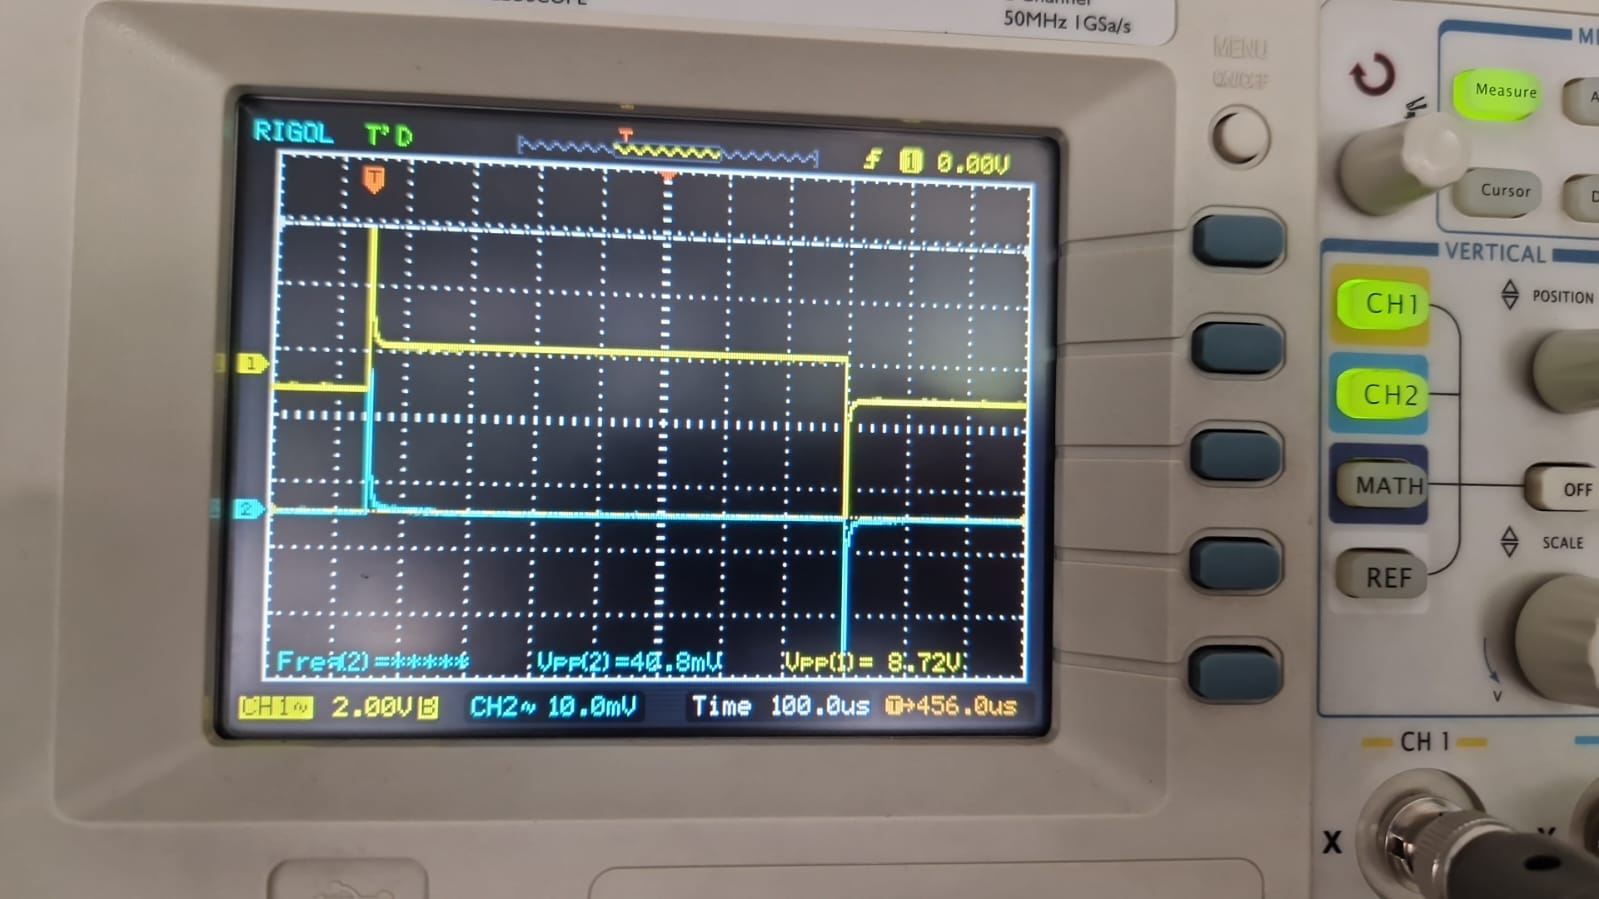
\includegraphics[width=0.9\textwidth]{assets/666-hz-5vpp.jpg}
    \caption{666Hz Output @ $5V_{pp}$}
    \label{fig:666-hz-5vpp-output}
\end{figure}

\begin{figure}[h]
    \centering
    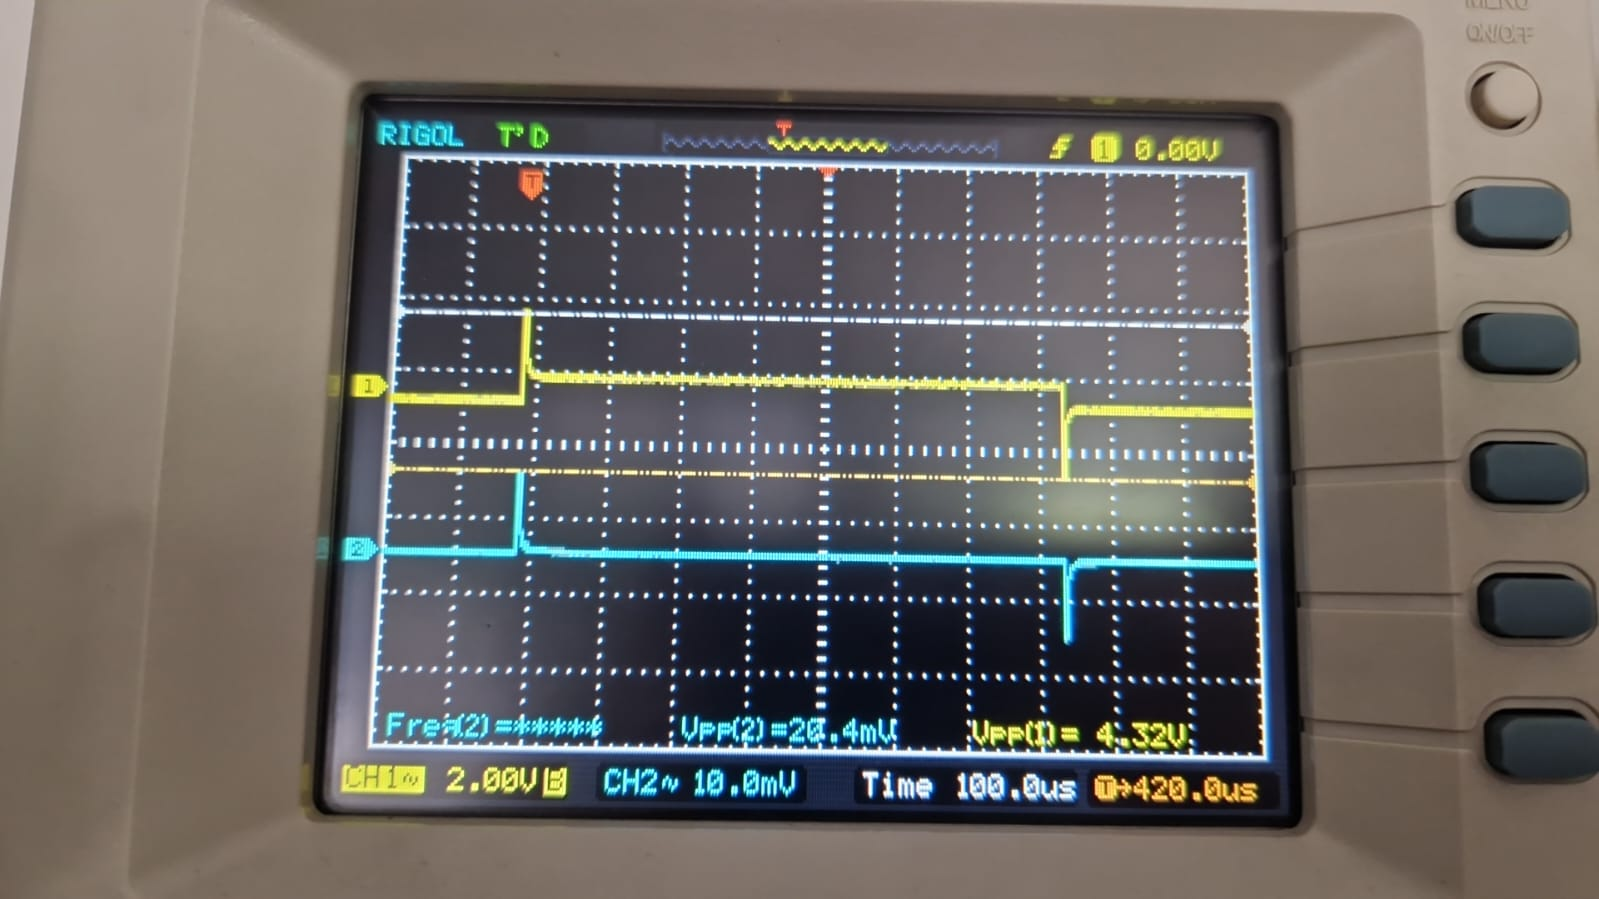
\includegraphics[width=0.9\textwidth]{assets/666-hz-2.5vpp.jpg}
    \caption{666Hz Output @ $2.5V_{pp}$}
    \label{fig:666-hz-2.5vpp-output}
\end{figure}

\begin{itemize}
    \item The period is long enough for the inductor to fully charge and discharge within each half-cycle.
    \item The voltage across the inductor shows a complete exponential rise and fall.
\end{itemize}

\newpage{}
\thispagestyle{plain}

\subsubsection{T=L/R $\implies$ f=6.66kHz}

\begin{figure}[h]
    \centering
    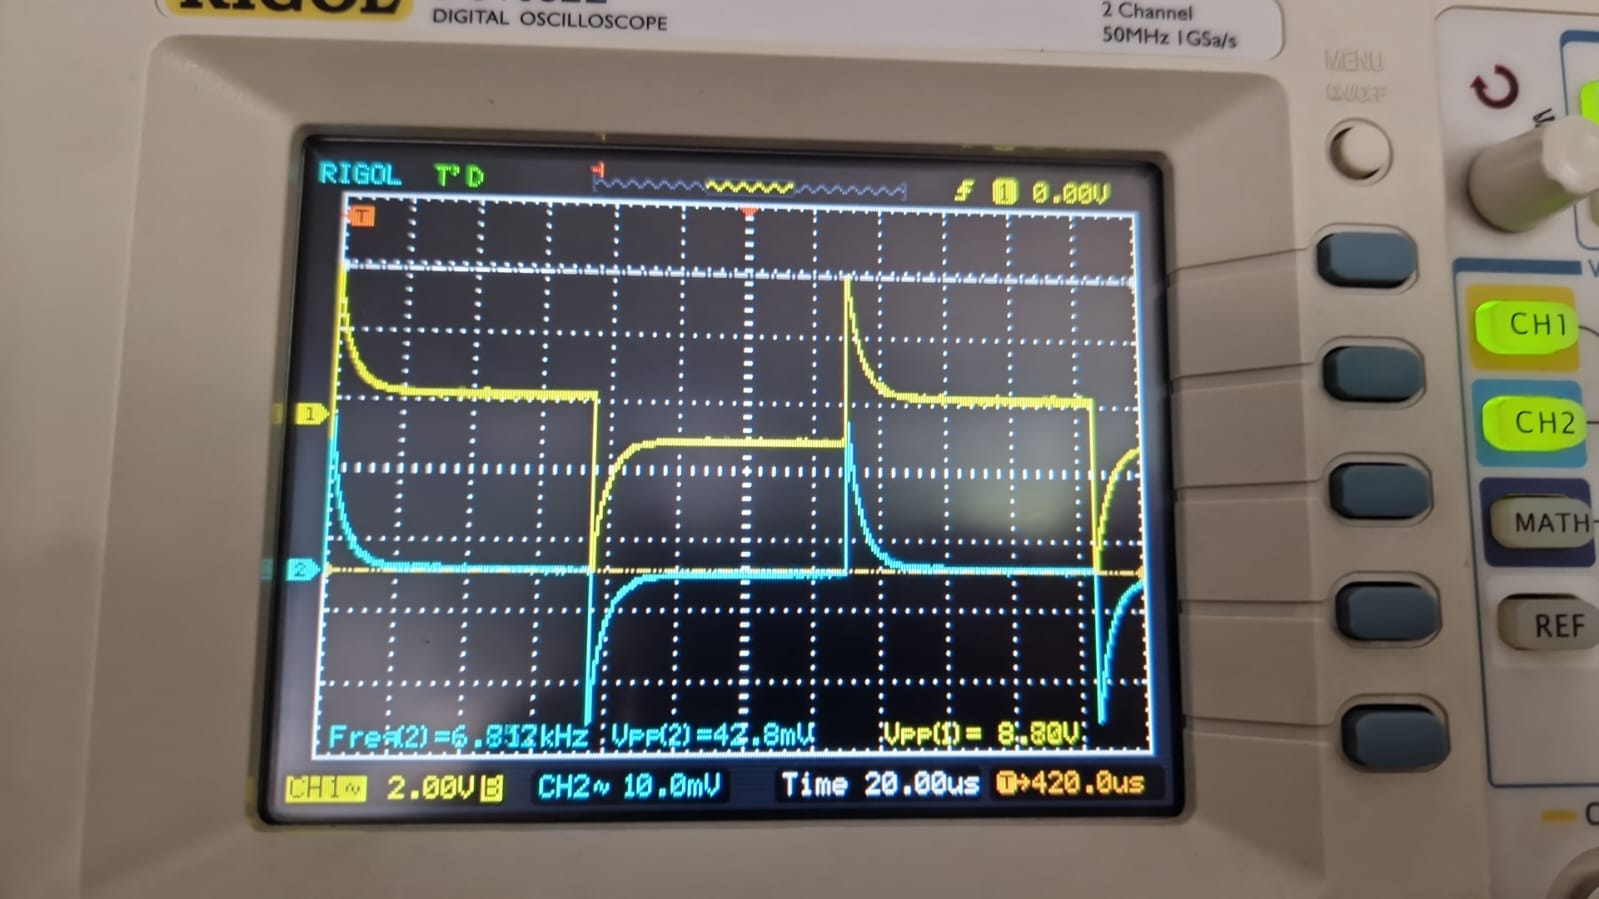
\includegraphics[width=0.9\textwidth]{assets/6666-hz-5vpp.jpg}
    \caption{6.66kHz Output @ $5V_{pp}$}
    \label{fig:6666-hz-5vpp-output}
\end{figure}

\begin{figure}[h]
    \centering
    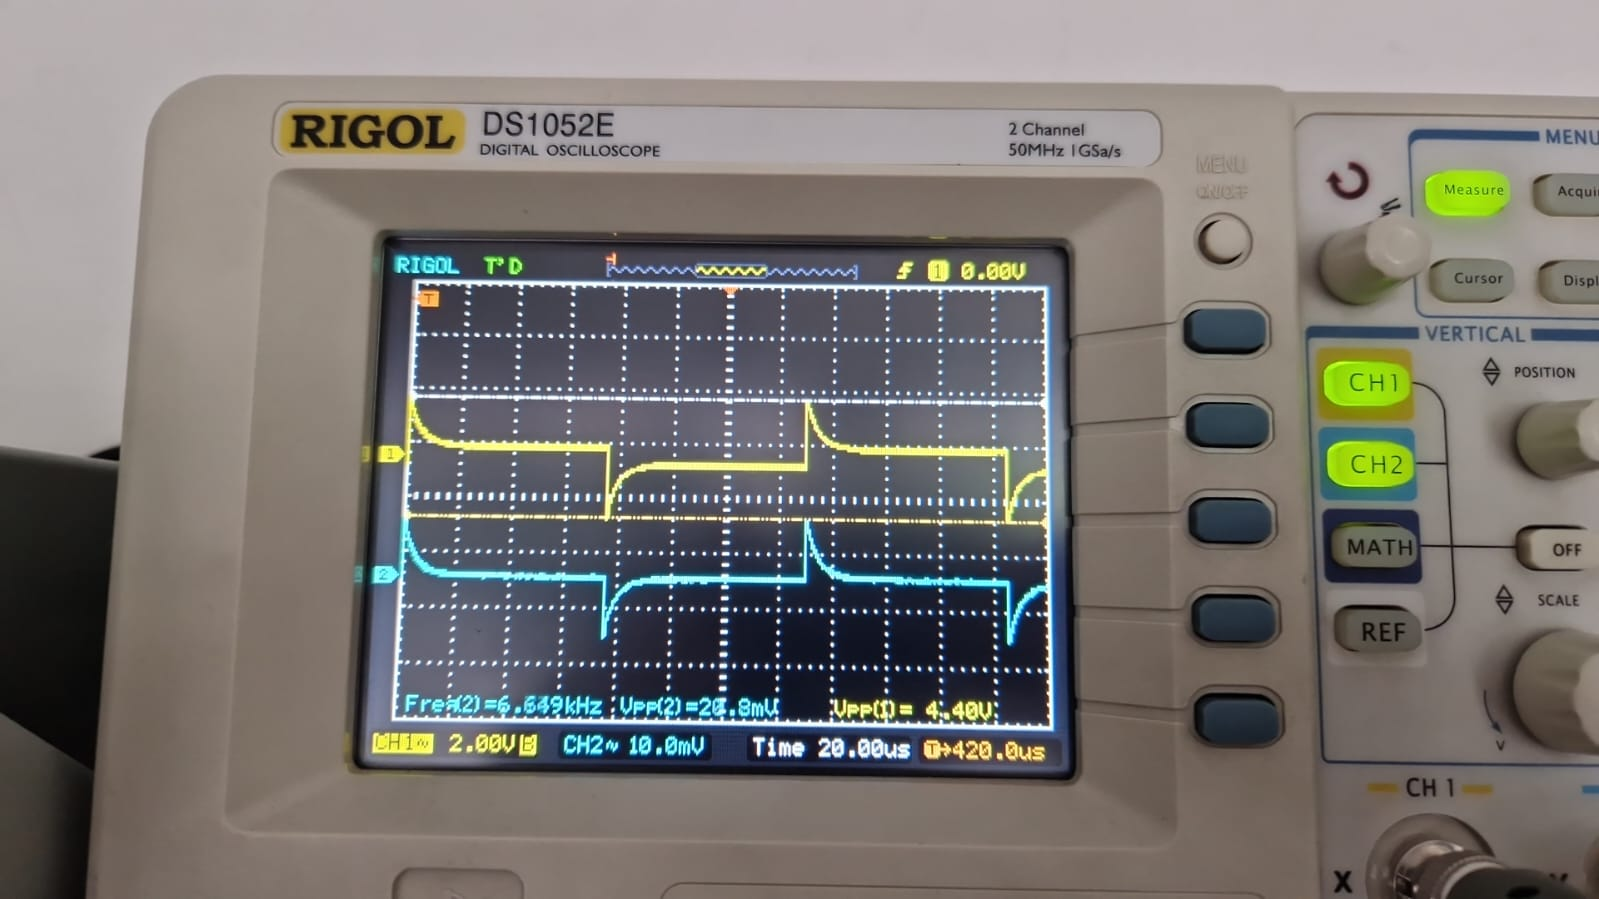
\includegraphics[width=0.9\textwidth]{assets/6666-hz-2.5vpp.jpg}
    \caption{6.66kHz Output @ $2.5V_{pp}$}
    \label{fig:6666-hz-2.5vpp-output}
\end{figure}

\begin{itemize}
    \item The period is equal to the time constant, allowing partial charging and discharging.
    \item The voltage across the inductor shows partial exponential rise and fall.
\end{itemize}

\newpage{}
\thispagestyle{plain}

\subsubsection{T=L/10R $\implies$ f=66.66kHz}

\begin{figure}[h]
    \centering
    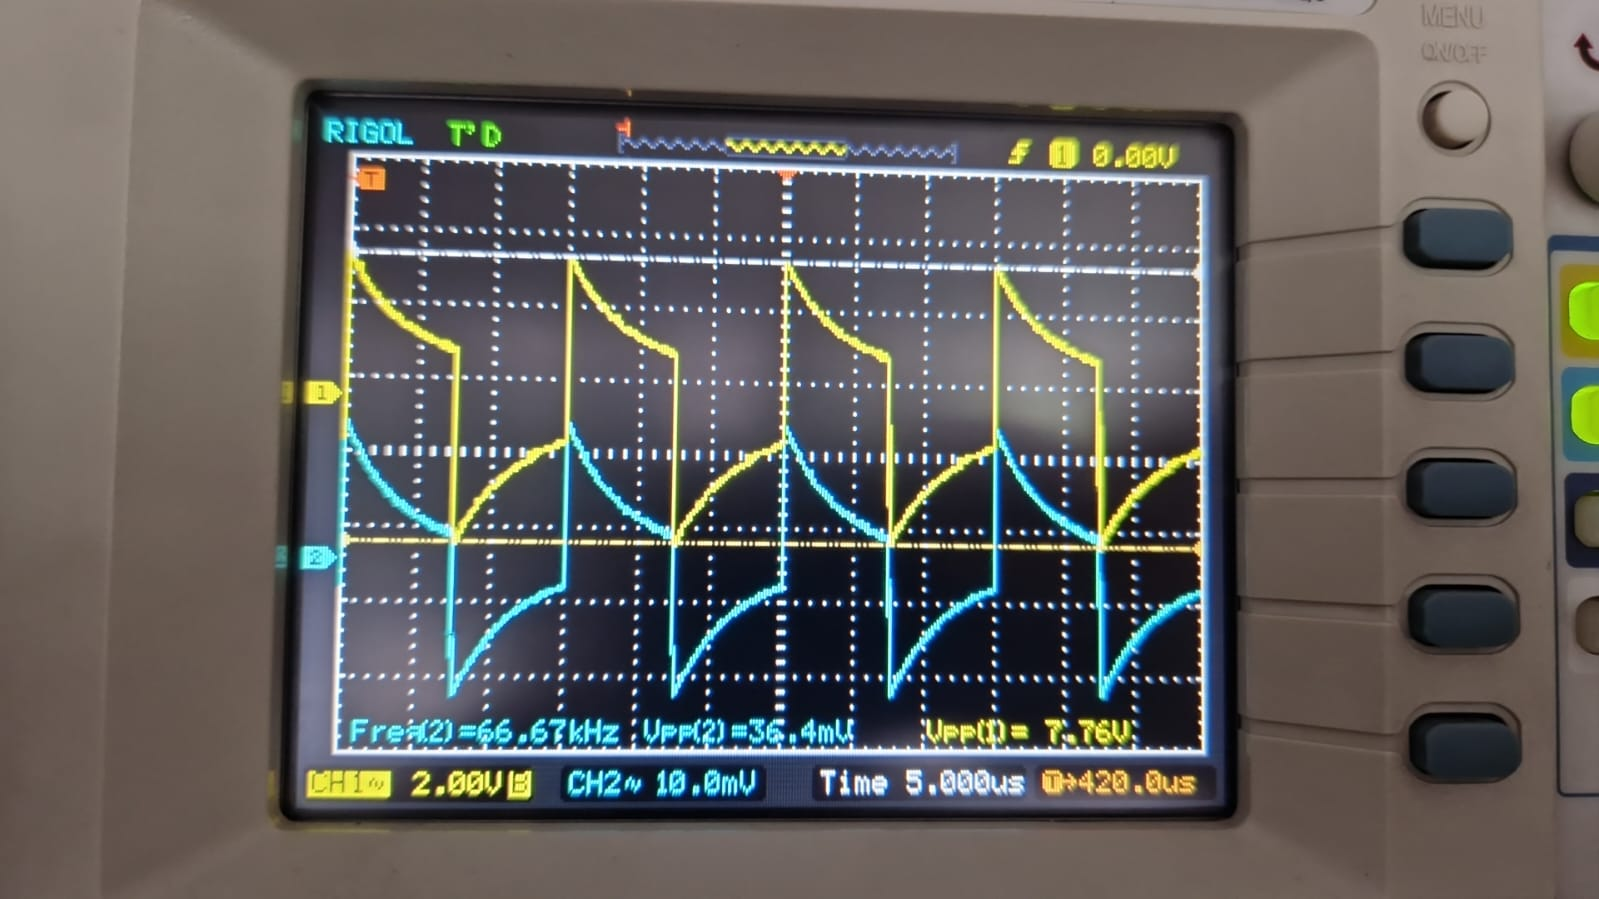
\includegraphics[width=0.9\textwidth]{assets/66666-hz-5vpp.jpg}
    \caption{66.66kHz Output @ $5V_{pp}$}
    \label{fig:66666-hz-5vpp-output}
\end{figure}

\begin{figure}[h]
    \centering
    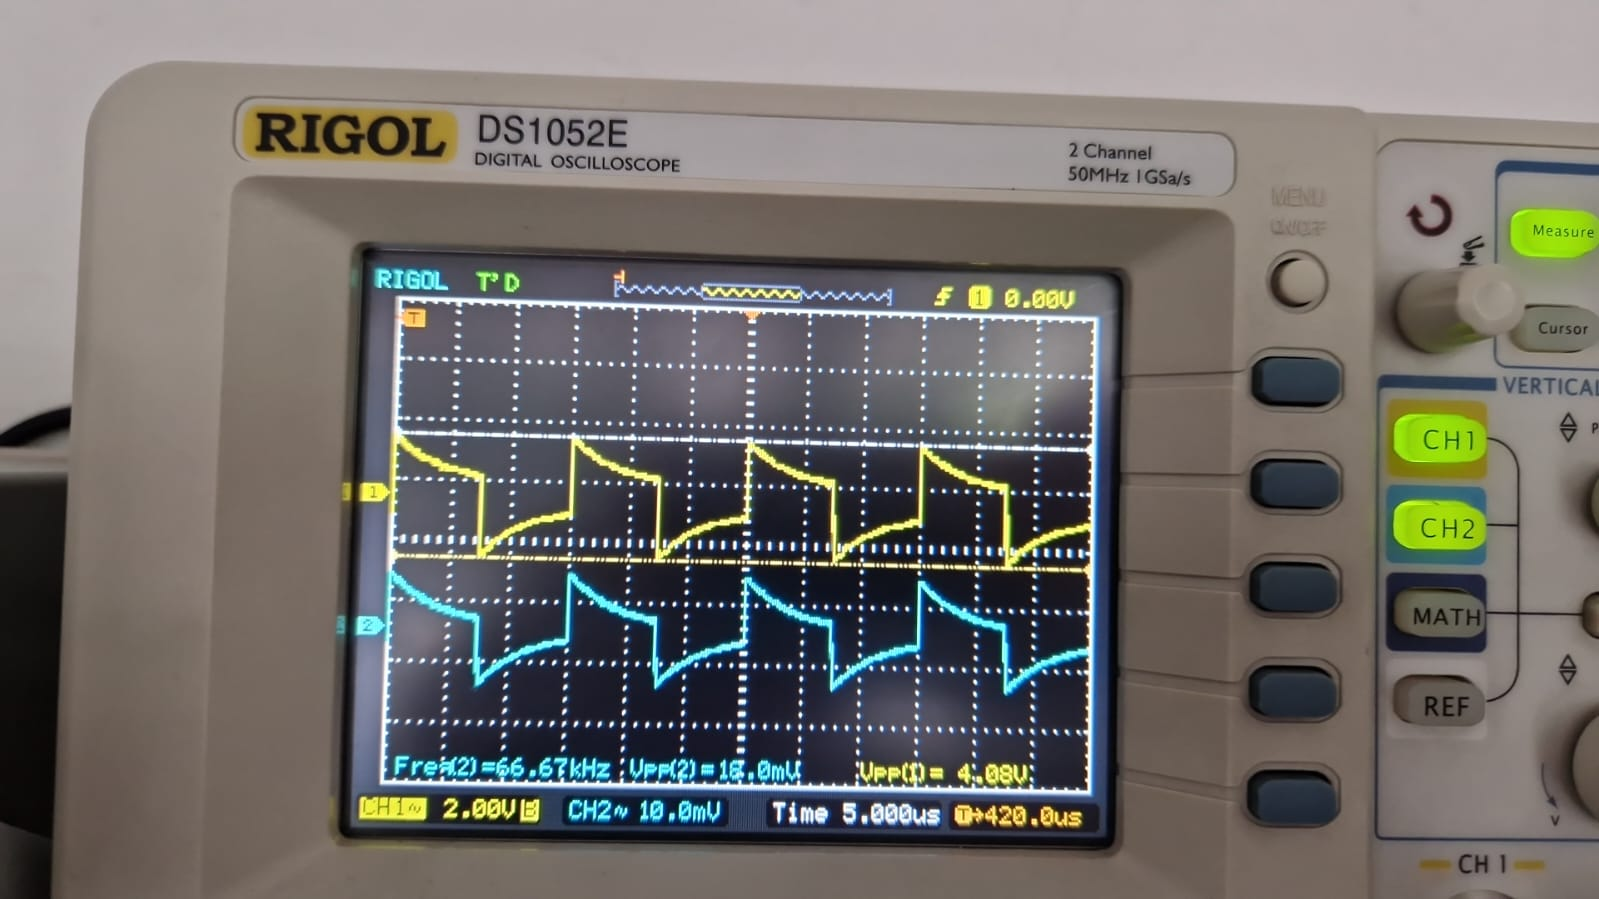
\includegraphics[width=0.9\textwidth]{assets/66666-hz-2.5vpp.jpg}
    \caption{66.66kHz Output @ $2.5V_{pp}$}
    \label{fig:66666-hz-2.5vpp-output}
\end{figure}

\begin{itemize}
    \item The period is very short, leading to minimal charging and discharging of the inductor.
    \item The voltage across the inductor barely shows any change.
\end{itemize}

\newpage{}
\thispagestyle{plain}

\subsubsection{Reducing the Amplitude}
When the amplitude of the square wave is reduced to half (0-2.5V), the voltages across both the inductor and the resistor also reduce proportionally. The overall behavior and response times remain consistent, but the magnitude of the voltages is halved.
